\documentclass{article}

\usepackage{color}
\usepackage[margin=1in]{geometry}
\usepackage{graphicx}
\usepackage{hyperref}
\usepackage{listings}

\definecolor{gray}{rgb}{0.5, 0.5, 0.5}
\definecolor{darkgreen}{rgb}{0, 0.6, 0}

\begin{document}
    \raggedright
    Homework 4 \break
    Christopher Seagraves
% % % % % % % % % % % % % % % % % % % % % % % % % % % % % % % % % % % % % % % % 

    \section*{Problem 1}
        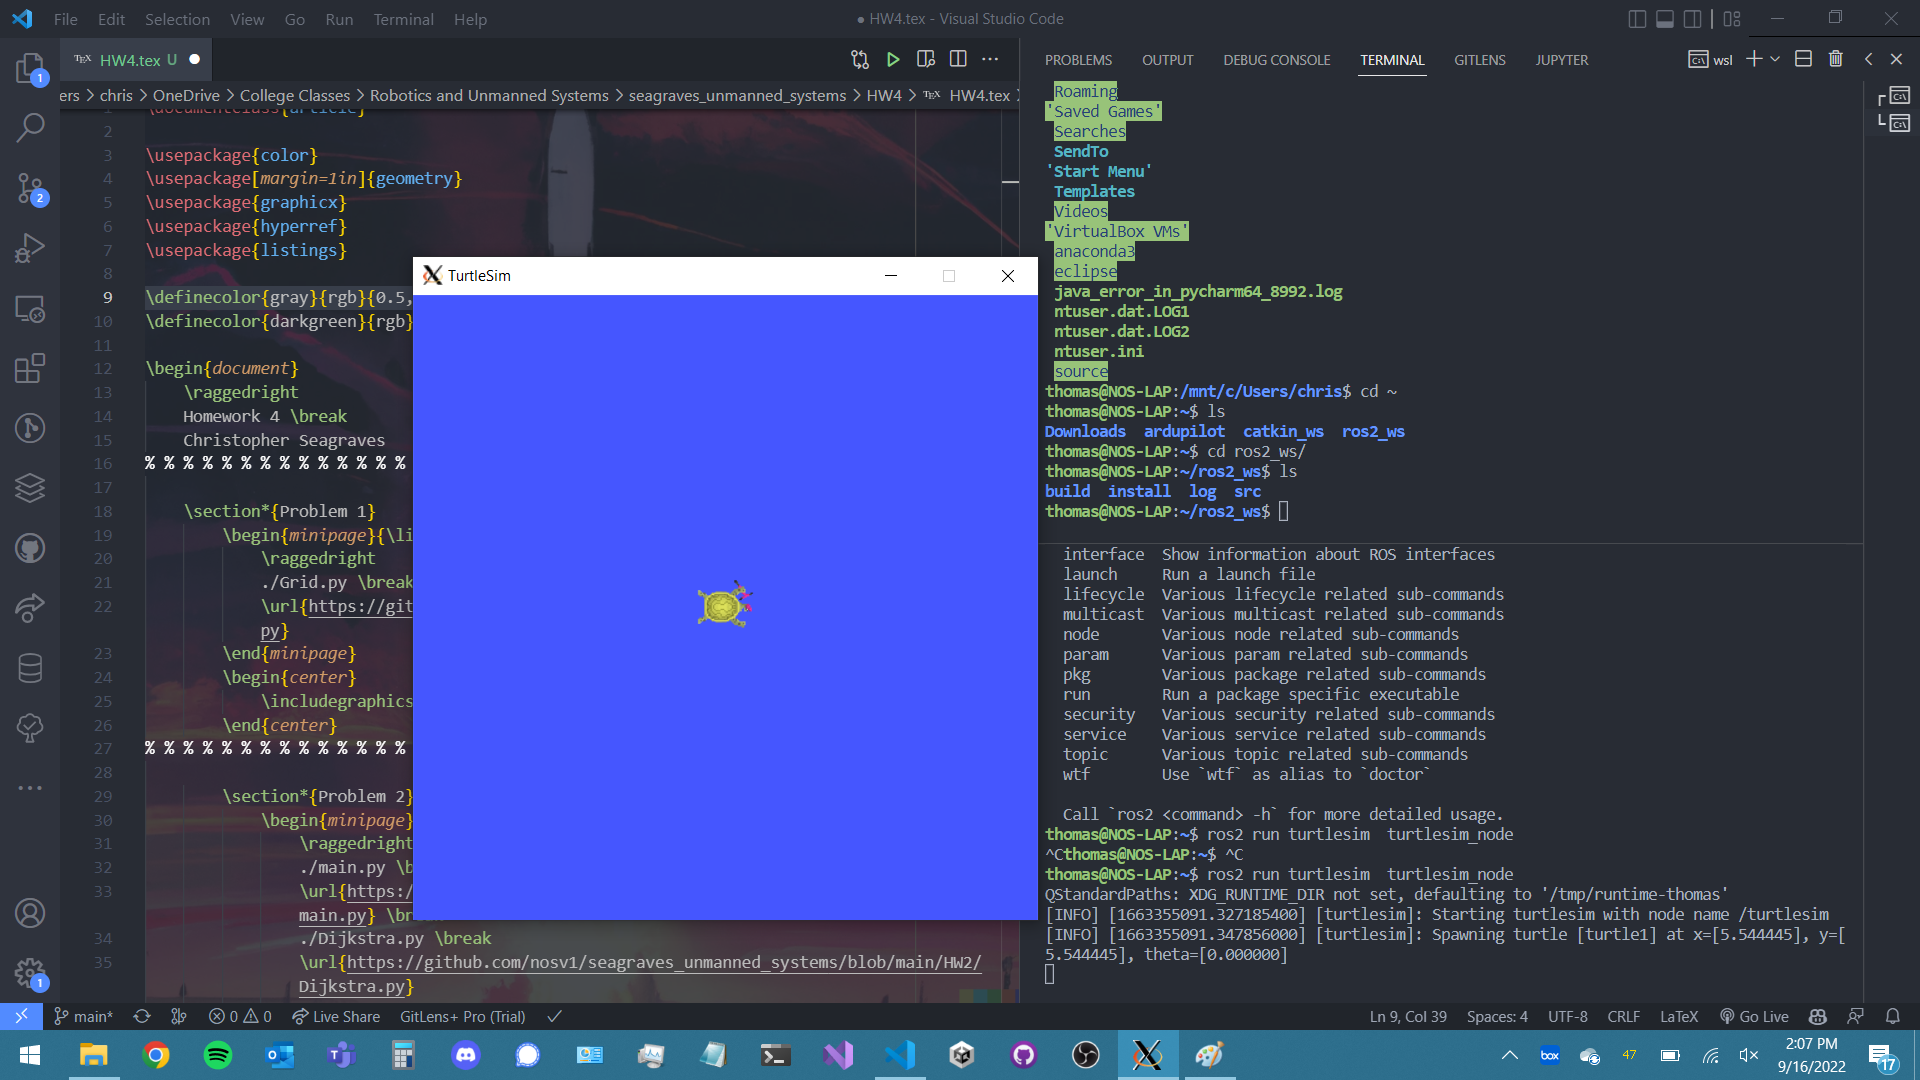
\includegraphics[width=\linewidth]{Problem 1 Turtlebot Simulator.png}
% % % % % % % % % % % % % % % % % % % % % % % % % % % % % % % % % % % % % % % %

    \section*{Problem 2}
        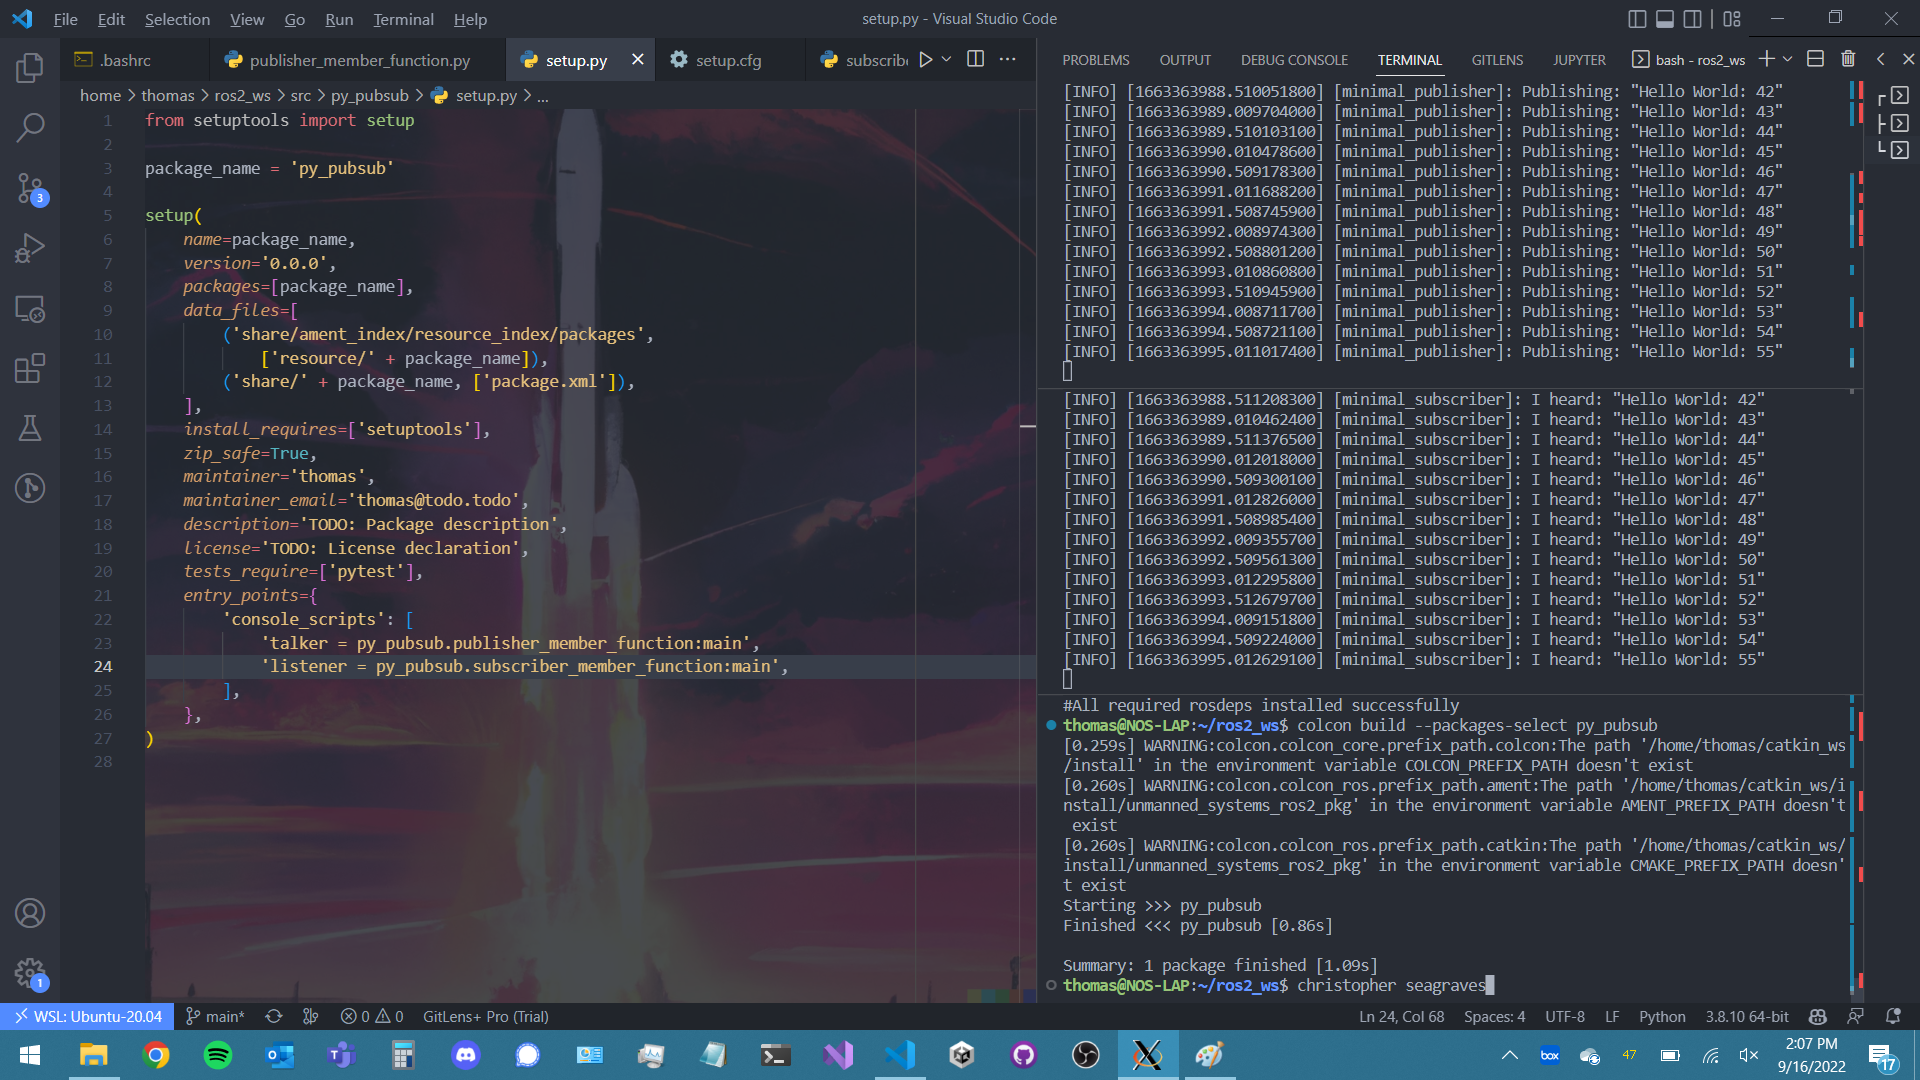
\includegraphics[width=\linewidth]{Problem 2 Publisher and Subscriber.png}
% % % % % % % % % % % % % % % % % % % % % % % % % % % % % % % % % % % % % % % %

    \section*{Problem 3}
        \raggedright
        controller.py \break
        \url{https://github.com/nosv1/seagraves_unmanned_systems_pkg/blob/master/seagraves_unmanned_systems_pkg/controller.py} \break
        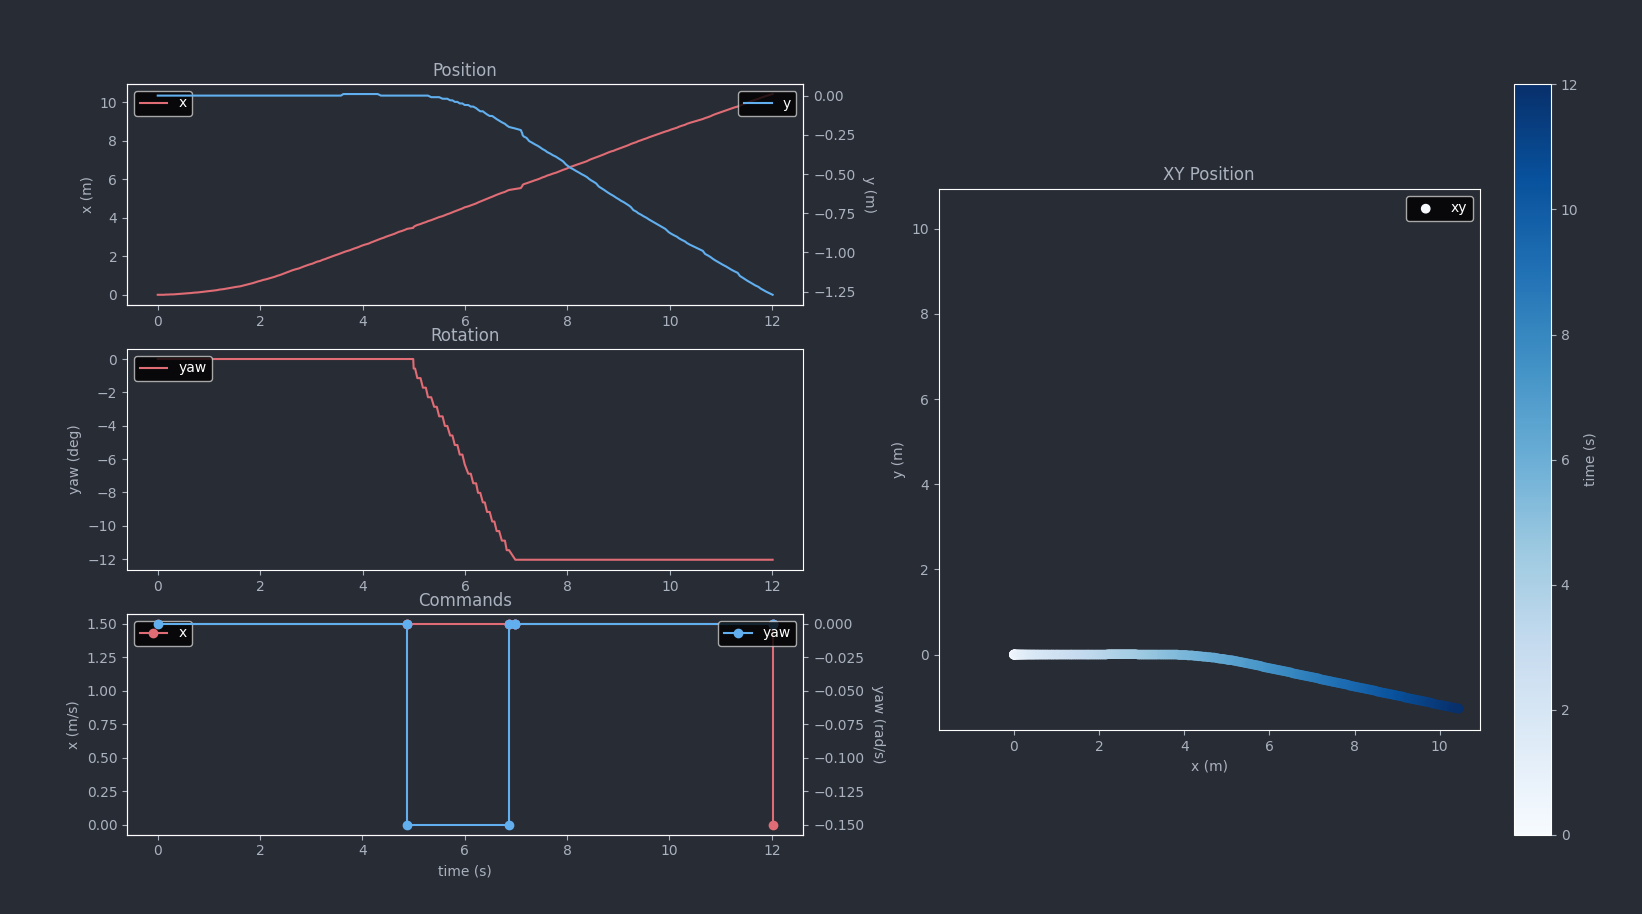
\includegraphics[width=\linewidth]{Problem 3 Telemetry.png}
% % % % % % % % % % % % % % % % % % % % % % % % % % % % % % % % % % % % % % % %
    
    \section*{Problem 4}
        \raggedright
        Kp = 6.5, Ki = 0.0, Kd = 0.0 \break
        Rise time = 0.6 seconds \break
        Given Burger can turn at 2.84 rad/s (162.4 deg/s), it can complete a 90 degree turn in 0.55 seconds - about .05 seconds per 10 degrees - so the optimal rise time would be about 0.44 seconds.
        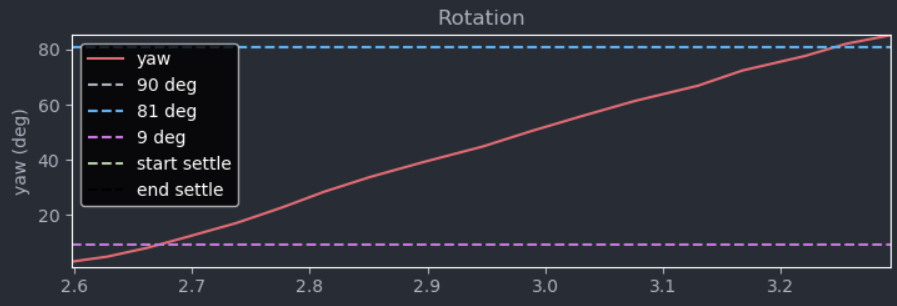
\includegraphics[width=\linewidth]{Problem 4 Rise Time.png} \break
        \begin{minipage}{\linewidth}
            \raggedright
            Settle time = 0.2 seconds \break
            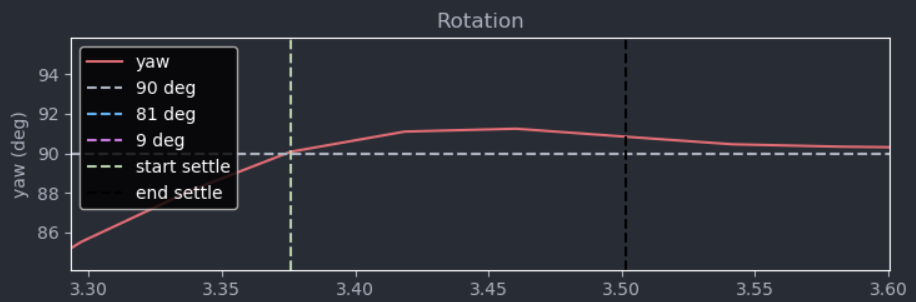
\includegraphics[width=\linewidth]{Problem 4 Settle Time.png} \break
        \end{minipage}
        \begin{minipage}{\linewidth}
            \raggedright
            Percent overshoot = 1\% 1 - (91.2 / 90) \break
            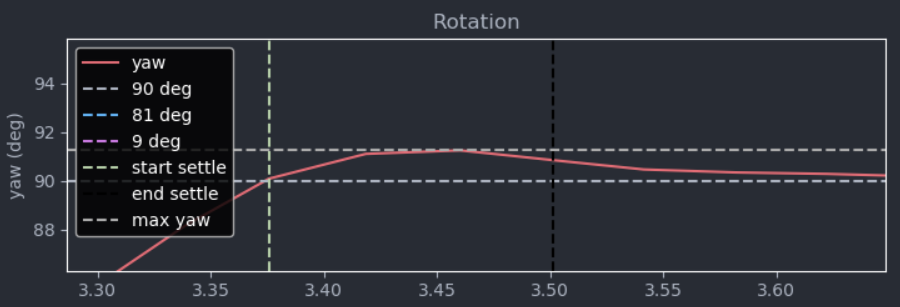
\includegraphics[width=\linewidth]{Problem 4 Percent Overshoot.png} \break
        \end{minipage}
        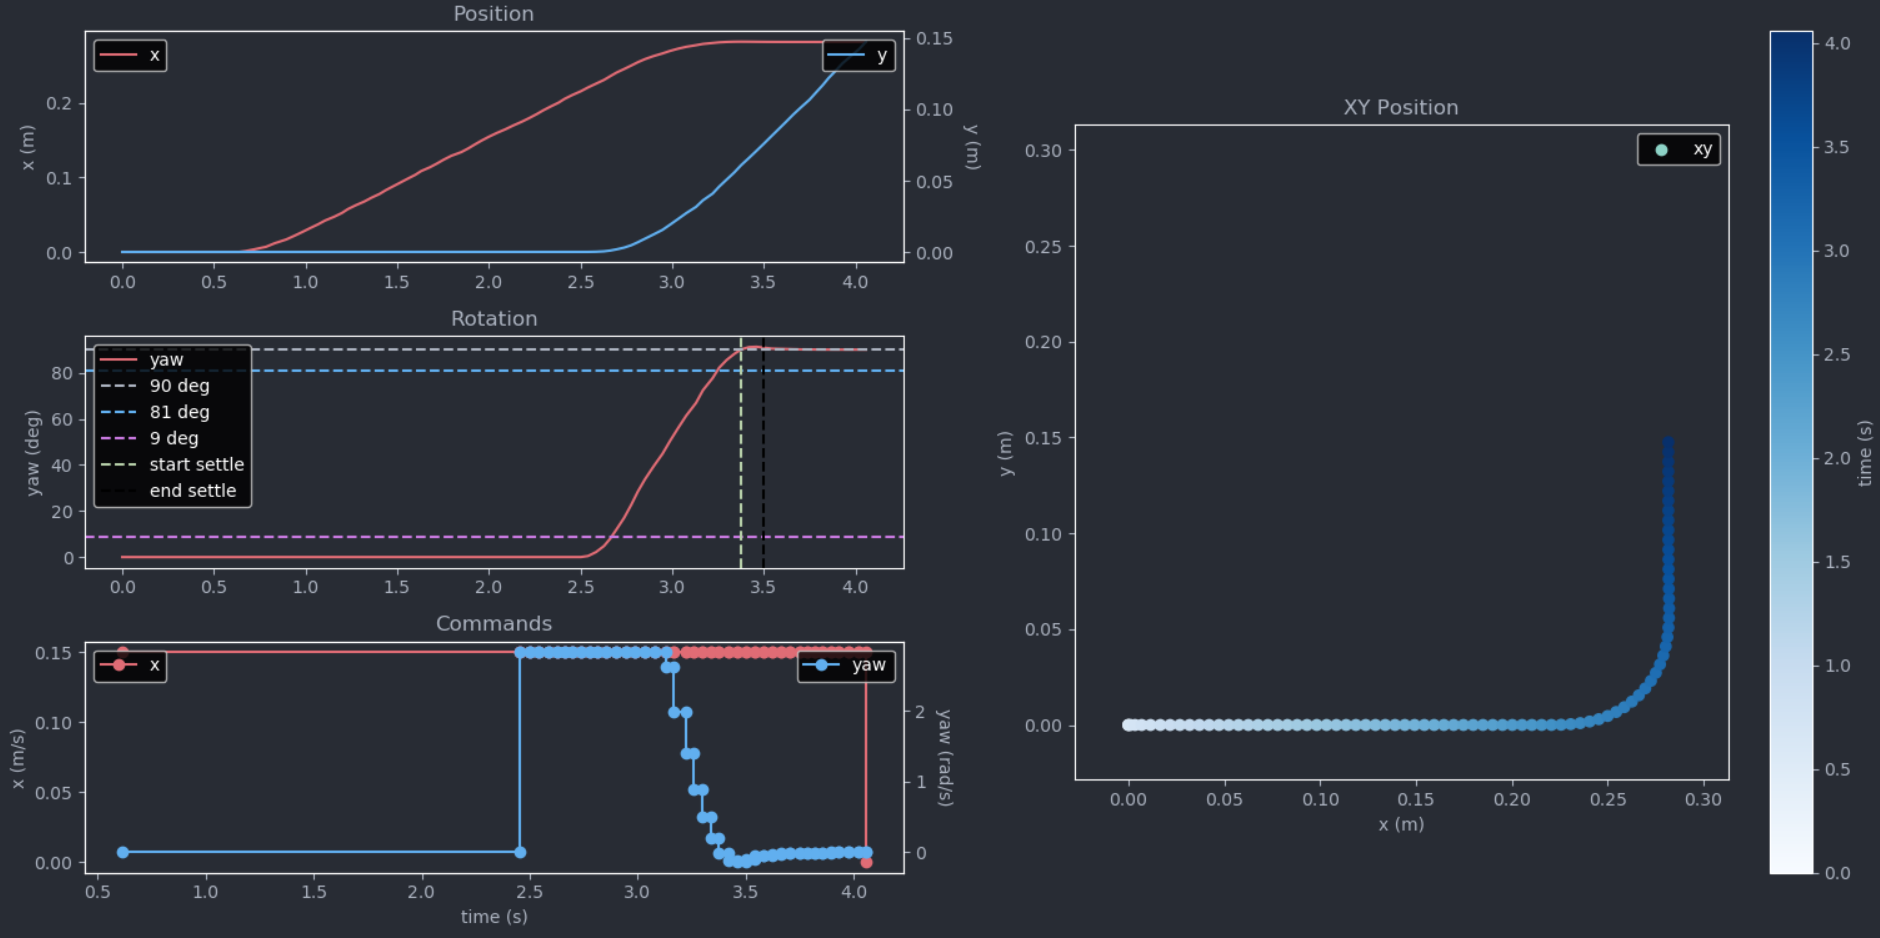
\includegraphics[width=\linewidth]{Problem 4 Telemetry.png}
% % % % % % % % % % % % % % % % % % % % % % % % % % % % % % % % % % % % % % % %

    \section*{Problem 5}
        \raggedright
        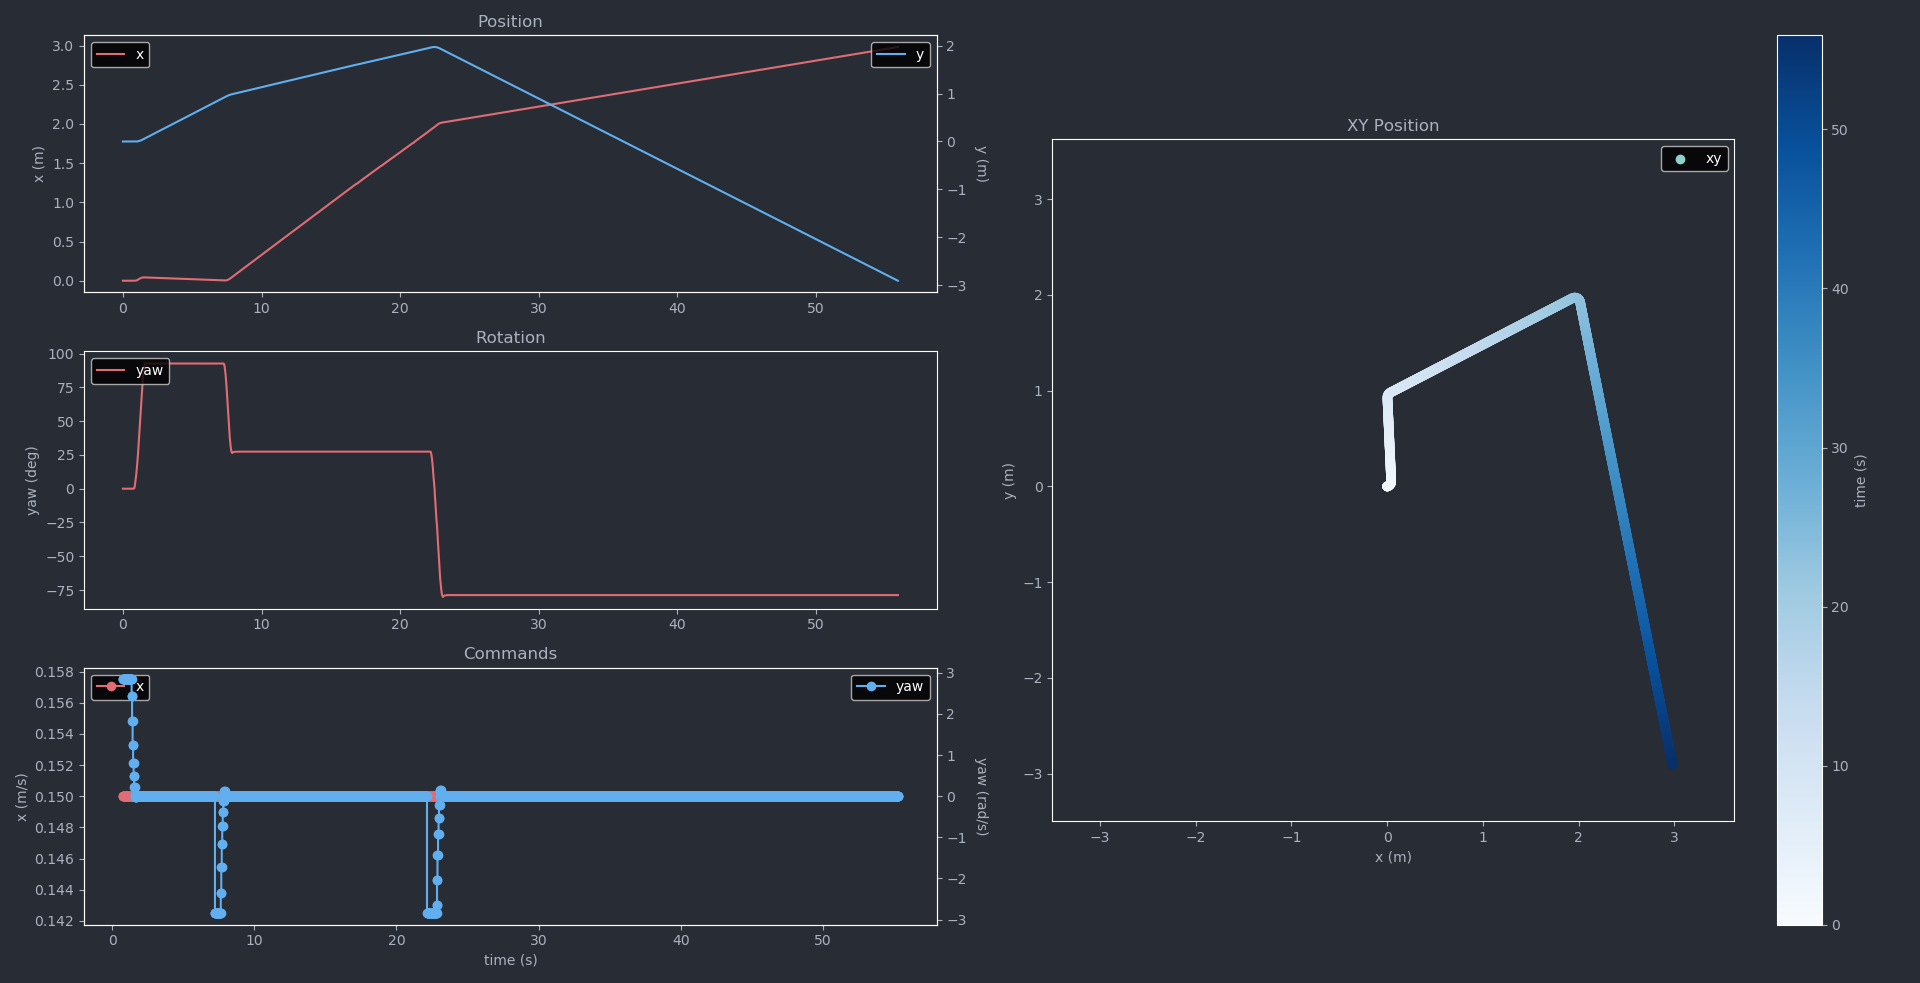
\includegraphics[width=\linewidth]{Problem 5 Telemetry.png}
% % % % % % % % % % % % % % % % % % % % % % % % % % % % % % % % % % % % % % % %

    \pagebreak
    \section*{Problem 6}
        \raggedright
        All runs below use the PID: kp=4.5, ki=0, kd=0.25 \break

        Clearly, as the speed increases, the PID controller is put under more stress; at 1.5m/s, this PID controller fails completley.
        Anything over 1 m/s and your pushing your luck, in my opinion. \break

        It would be cool to have a PID controller for throttle that also takes into consideration the heading error so it could maybe slow down if it detected error and pedal to the medal otherwise... but this still wouldn't solve the overshoot problem compeltley; you would need a method to know how fast you could turn and slow down for the next 'big step' in optimality. \break

        \begin{minipage}{\linewidth}
            \raggedright
            Speed: 0.15 m/s \break
            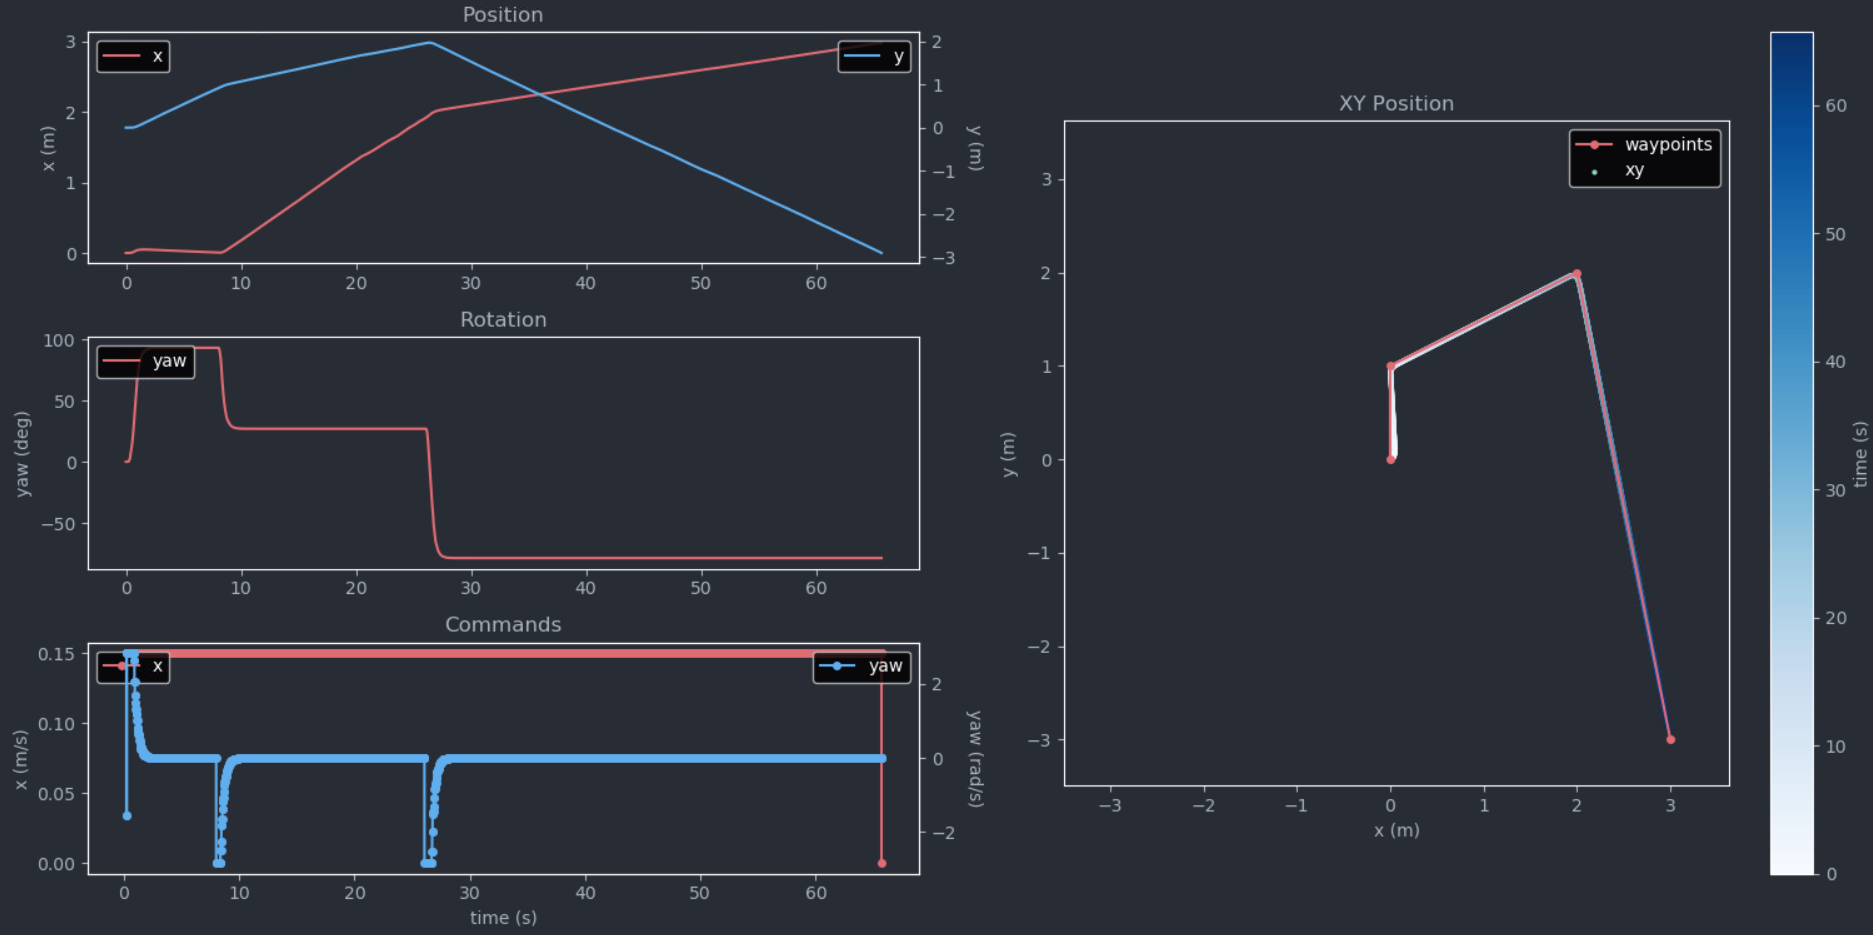
\includegraphics[width=5in]{Problem 6 Telemetry 0o15.png} \break
        \end{minipage}

        \begin{minipage}{\linewidth}
            \raggedright
            Speed: 0.6 m/s \break
            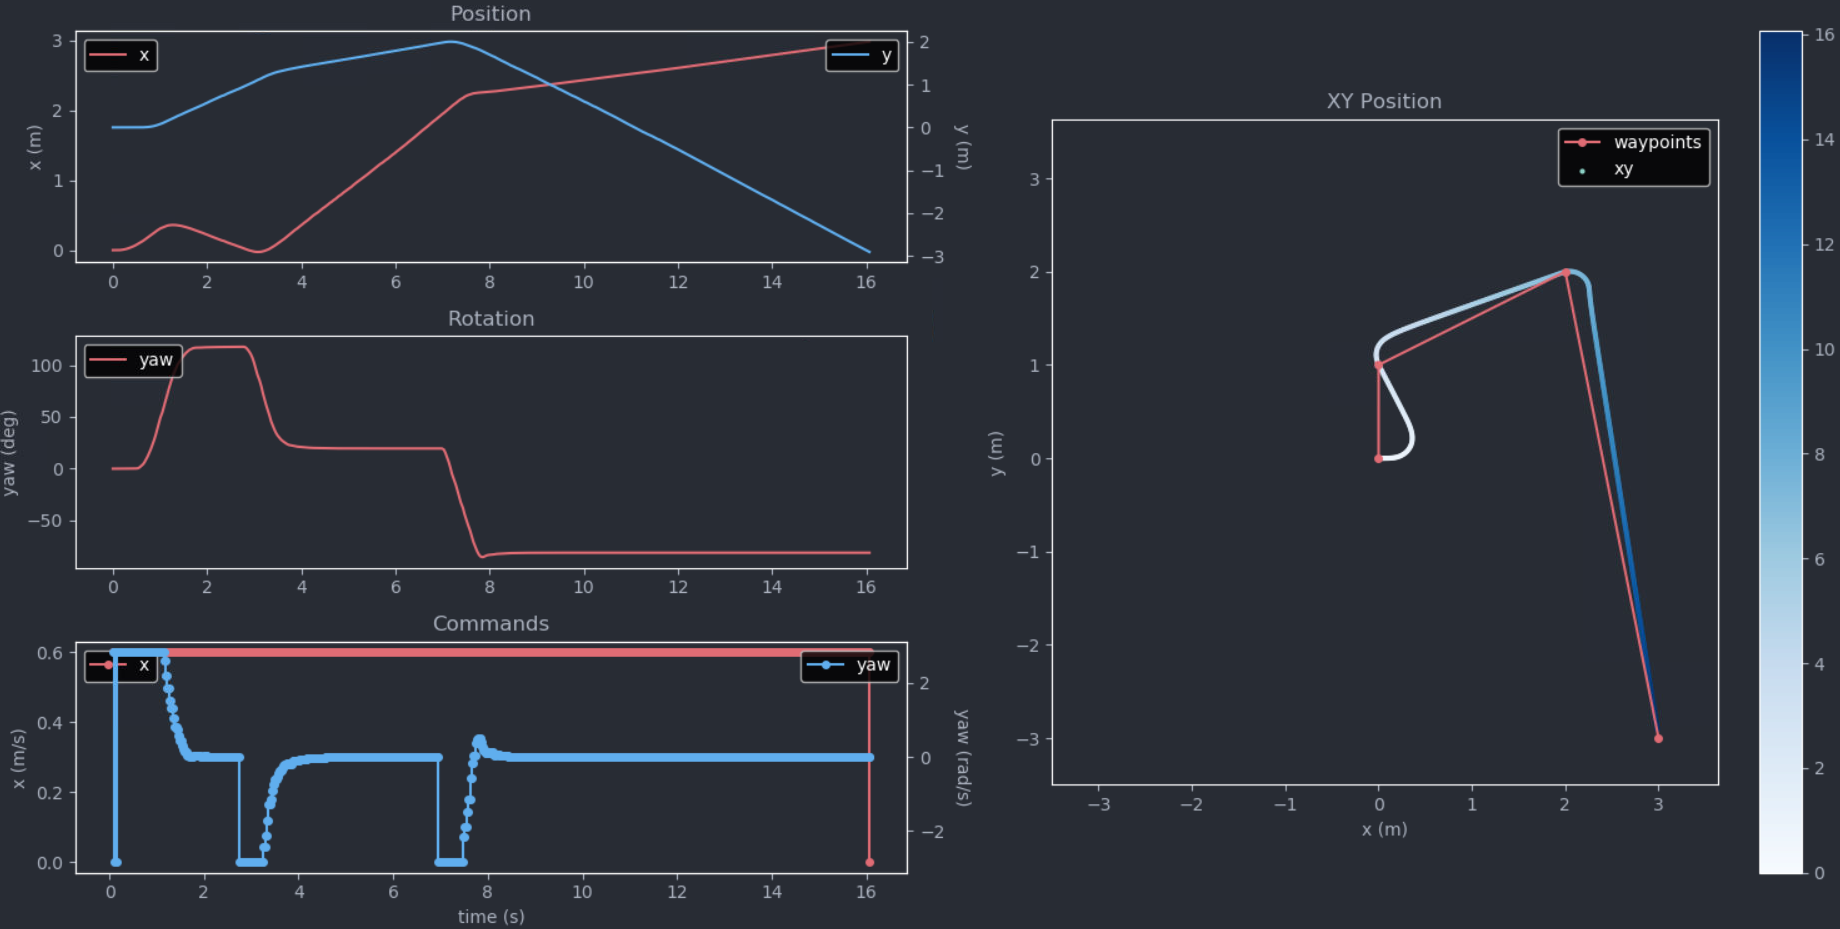
\includegraphics[width=5in]{Problem 6 Telemetry 0o6.png} \break
        \end{minipage}

        \begin{minipage}{\linewidth}
            \raggedright
            Speed: 1.05 m/s \break
            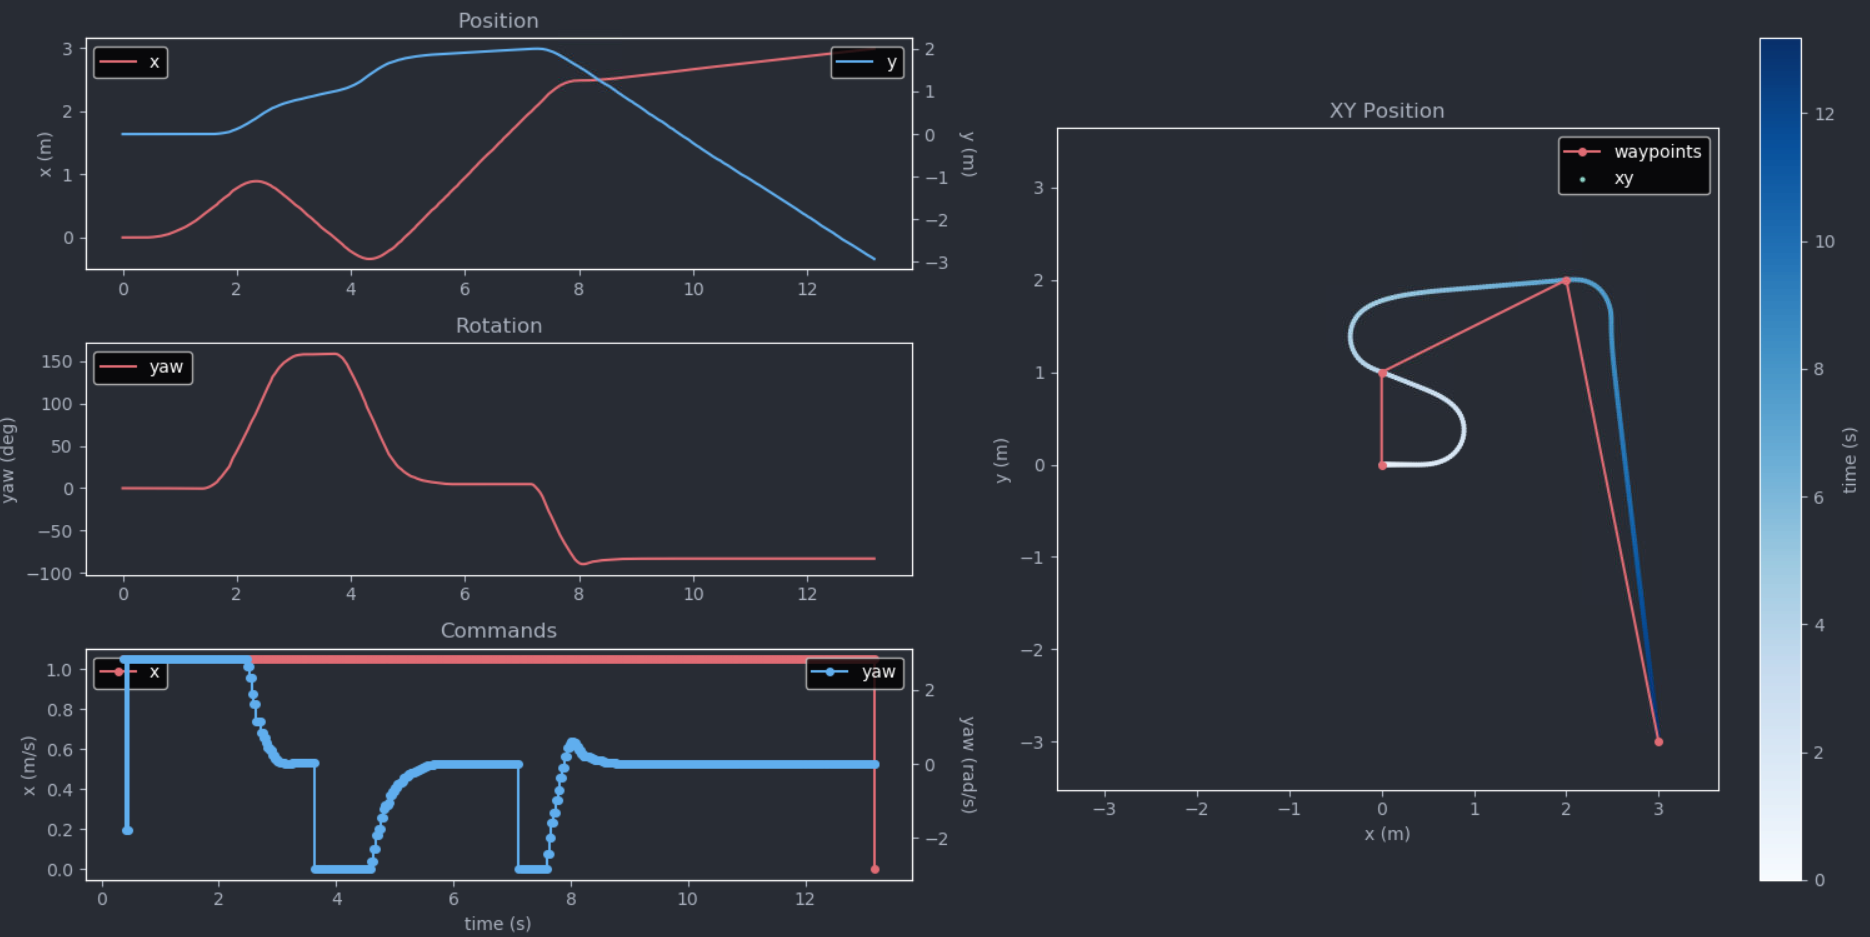
\includegraphics[width=5in]{Problem 6 Telemetry 1o05.png} \break        
        \end{minipage}

        \begin{minipage}{\linewidth}
            \raggedright
            Speed: 1.5 m/s \break
            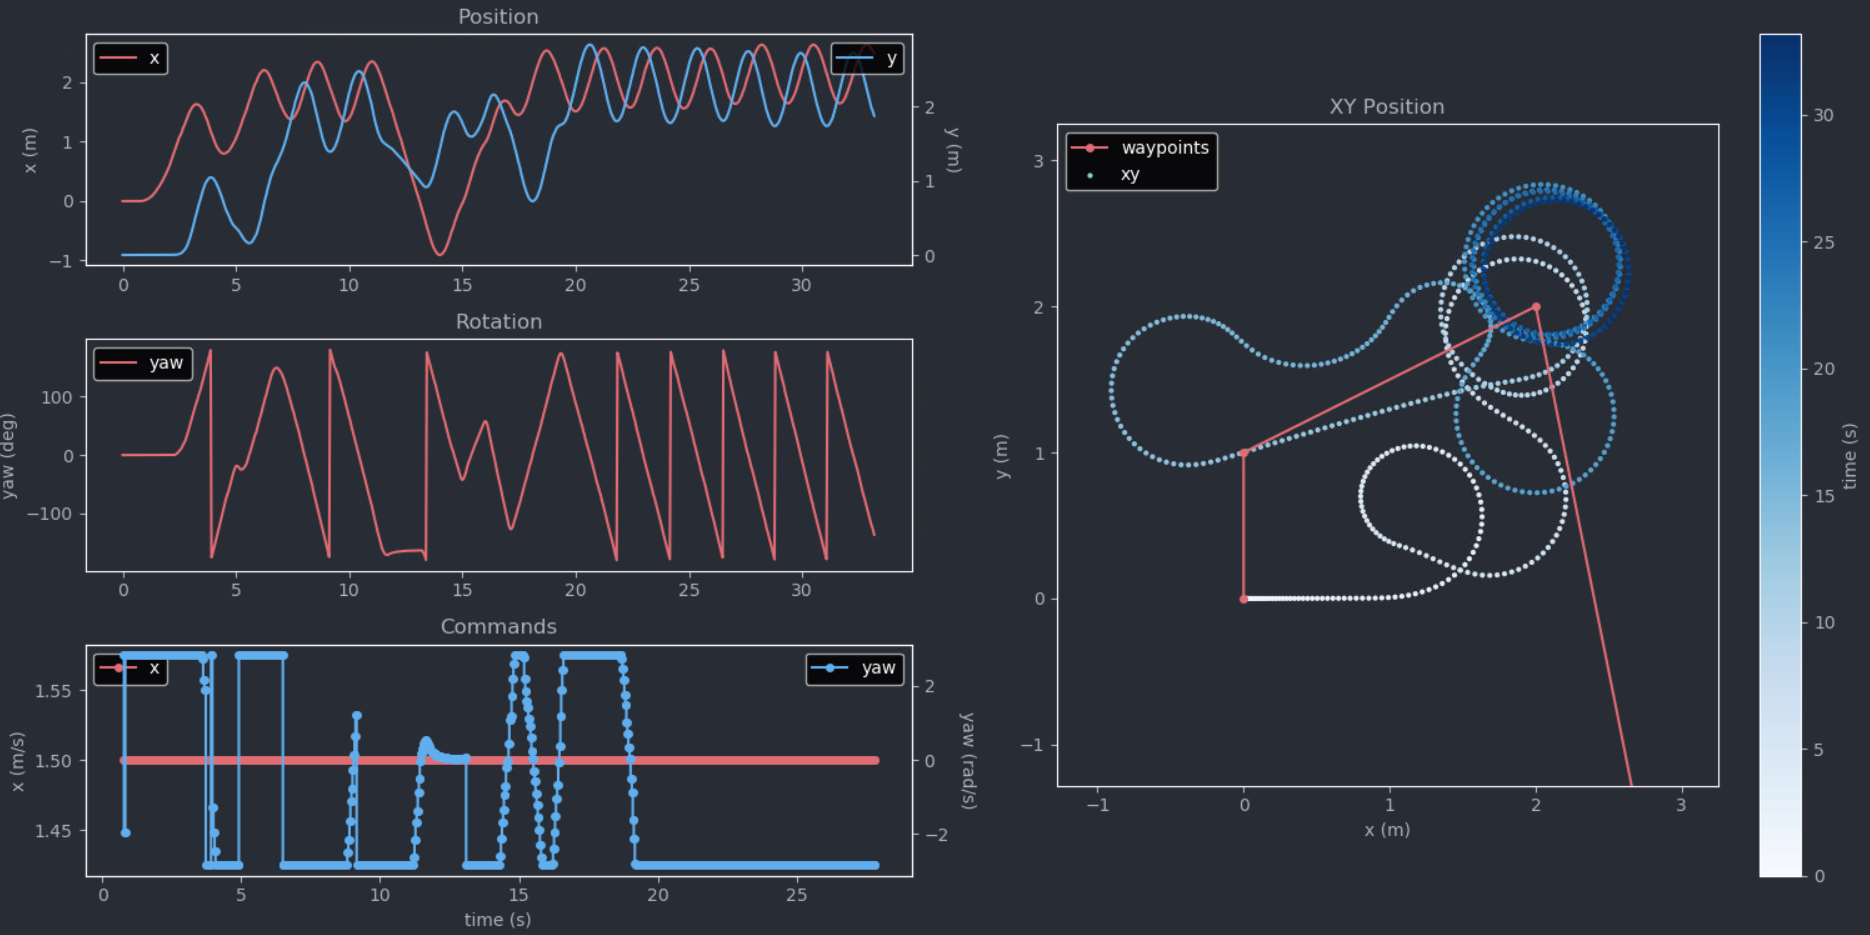
\includegraphics[width=5in]{Problem 6 Telemetry 1o5.png} \break
        \end{minipage}
% % % % % % % % % % % % % % % % % % % % % % % % % % % % % % % % % % % % % % % %

    \pagebreak
    \section*{Notes}
    Personal imports can be found in the 'support\_module' directory \break
    Log plotter can be found in 'extra' directory \break

    You may notice the additional package directory, 'turtlebot3\_gazebo'. Mainly used in the 'Rapid Simulations' branch (working on GA stuff for fun), I edited the oringal worlds to run in headless mode and/or speed up simulations, had to edit /worlds/empty\_worlds/burger.model and /launch/empty\_world\_no\_x\_launch.py

\end{document}